% ============================================================
%  Preparatório OBI — Aula 03
%  Fila (Queue) e Fila de Prioridade (Priority Queue)
%  Grupo: GEMA
%  Compilar: pdflatex aula03_queue.tex  (2x para refs)
% ============================================================
\documentclass[aspectratio=169,10pt]{beamer}

\usetheme{Madrid}
\usecolortheme{default}

% ── Pacotes ───────────────────────────────────────────────
\usepackage[utf8]{inputenc}
\usepackage[T1]{fontenc}
\usepackage[english]{babel}
\usepackage{graphicx}
\usepackage{listings}
\usepackage{xcolor}
\usepackage{tikz}
\usepackage{amsmath}
\usepackage{tcolorbox}
\usepackage{array}
\usepackage{booktabs}
\usepackage{adjustbox}
\tcbuselibrary{skins,breakable,listings}
\usetikzlibrary{arrows.meta,shapes,positioning,fit,calc,
                decorations.pathreplacing,backgrounds}

% ── Margens apertadas para caber mais conteudo ────────────
\setbeamersize{text margin left=4mm,text margin right=4mm}
\setlength{\leftmargini}{1.0em}
\setlength{\leftmarginii}{0.9em}

% ── Paleta de cores ───────────────────────────────────────
\definecolor{gemaBlue}   {RGB}{13,  43,  90}
\definecolor{gemaCyan}   {RGB}{0,  170, 210}
\definecolor{gemaRed}    {RGB}{190, 30,  30}
\definecolor{gemaOrange} {RGB}{220, 110,  0}
\definecolor{codeBack}   {RGB}{22,  27,  34}
\definecolor{codeGreen}  {RGB}{80,  200, 120}
\definecolor{codeBlue}   {RGB}{121, 192, 255}
\definecolor{codeYellow} {RGB}{255, 210,  70}
\definecolor{codeOrange} {RGB}{255, 160,  60}
\definecolor{alertYellow}{RGB}{255, 243, 176}
\definecolor{alertBorder}{RGB}{160, 110,   0}
\definecolor{queueColor} {RGB}{0,  140, 180}
\definecolor{pqColor}    {RGB}{130,  0, 170}
\definecolor{nodeGreen}  {RGB}{30,  150,  80}

% ── Cores Beamer ──────────────────────────────────────────
\setbeamercolor{palette primary}    {bg=gemaBlue,fg=white}
\setbeamercolor{palette secondary}  {bg=gemaBlue!85,fg=white}
\setbeamercolor{palette tertiary}   {bg=gemaBlue!65,fg=white}
\setbeamercolor{palette quaternary} {bg=gemaBlue,fg=white}
\setbeamercolor{structure}          {fg=gemaBlue}
\setbeamercolor{frametitle}         {fg=white,bg=gemaBlue}
\setbeamercolor{block title}        {fg=white,bg=gemaBlue}
\setbeamercolor{block body}         {fg=black,bg=gemaBlue!7}
\setbeamercolor{block title alerted}{fg=white,bg=gemaRed}
\setbeamercolor{block body alerted} {fg=black,bg=gemaRed!8}
\setbeamercolor{block title example}{fg=white,bg=gemaCyan!75!black}
\setbeamercolor{block body example} {fg=black,bg=gemaCyan!10}
\setbeamercolor{itemize item}       {fg=gemaCyan!70!black}
\setbeamercolor{itemize subitem}    {fg=gemaBlue!60}

\setbeamerfont{frametitle}{size=\large,series=\bfseries}
\setbeamertemplate{navigation symbols}{}

% ── Rodapé ────────────────────────────────────────────────
\setbeamertemplate{footline}{%
  \leavevmode\hbox{%
    \begin{beamercolorbox}[wd=.33\paperwidth,ht=2.8ex,dp=1.2ex,center]{palette secondary}
      \tiny GEMA
    \end{beamercolorbox}%
    \begin{beamercolorbox}[wd=.34\paperwidth,ht=2.8ex,dp=1.2ex,center]{palette primary}
      \tiny Queue
    \end{beamercolorbox}%
    \begin{beamercolorbox}[wd=.33\paperwidth,ht=2.8ex,dp=1.2ex,right]{palette secondary}
      \tiny \insertframenumber/\inserttotalframenumber\hspace{2mm}
    \end{beamercolorbox}%
  }%
}

% ── Estilo de codigo C++ (padrao) ─────────────────────────
\lstdefinestyle{cppstyle}{
  language=C++,
  backgroundcolor=\color{codeBack},
  basicstyle=\ttfamily\scriptsize\color{white},
  keywordstyle=\color{codeBlue}\bfseries,
  stringstyle=\color{codeOrange},
  commentstyle=\color{codeGreen}\itshape,
  numberstyle=\tiny\color{gray!60},
  identifierstyle=\color{white},
  morekeywords={queue,priority_queue,stack,vector,pair,greater,bool,auto,long},
  emph={push,pop,front,back,top,empty,size,cin,cout,min,max,make_pair},
  emphstyle=\color{codeYellow}\bfseries,
  numbers=left, numbersep=5pt,
  frame=none, tabsize=4,
  showstringspaces=false,
  breaklines=true, columns=flexible, keepspaces=true,
  xleftmargin=10pt,
  aboveskip=0pt, belowskip=0pt,
}

% ── Estilo minusculo para slides densos ───────────────────
\lstdefinestyle{cppsmall}{
  style=cppstyle,
  basicstyle=\ttfamily\tiny\color{white},
  numberstyle=\tiny\color{gray!50},
  numbersep=3pt,
  xleftmargin=7pt,
  lineskip=-1pt,
}

% ── Caixas tcolorbox ──────────────────────────────────────
\tcbset{
  before skip=1pt, after skip=1pt, boxsep=0pt,
  caixaBase/.style={
    enhanced, arc=4pt, boxrule=0.8pt,
    left=3pt, right=3pt, top=2pt, bottom=2pt,
    fonttitle=\bfseries\footnotesize,
  },
  caixaAzul/.style={caixaBase,
    colback=gemaBlue!6, colframe=gemaBlue},
  caixaVerde/.style={caixaBase,
    colback=codeGreen!8, colframe=codeGreen!55!black,
    fonttitle=\bfseries\footnotesize\color{codeGreen!35!black}},
  caixaVermelho/.style={caixaBase,
    colback=gemaRed!8, colframe=gemaRed,
    fonttitle=\bfseries\footnotesize\color{gemaRed!80!black}},
  caixaLaranja/.style={caixaBase,
    colback=gemaOrange!8, colframe=gemaOrange,
    fonttitle=\bfseries\footnotesize\color{gemaOrange!80!black}},
  caixaRoxa/.style={caixaBase,
    colback=pqColor!8, colframe=pqColor!70,
    fonttitle=\bfseries\footnotesize\color{pqColor!70!black}},
  caixaAmarelo/.style={caixaBase,
    colback=alertYellow, colframe=alertBorder,
    fonttitle=\bfseries\footnotesize\color{alertBorder}},
  caixaCodigo/.style={
    enhanced, arc=4pt, boxrule=0.8pt,
    colback=codeBack, colframe=gemaCyan!45,
    left=1pt, right=1pt, top=1pt, bottom=1pt},
}

% ── Metadados ─────────────────────────────────────────────
\title[Aula 03 --- Queue]{Fila e Fila de Prioridade}
\subtitle{Preparatorio OBI --- Aula 03}
\author[GEMA]{Grupo de Extensao em Maratonas de Programação}
\institute{GEMA}
\date{2025}

% =============================================================
\begin{document}
% =============================================================

% ─────────────────────────────────────────────────────────────
%  SLIDE DE TITULO
% ─────────────────────────────────────────────────────────────
{
\setbeamertemplate{footline}{}
\begin{frame}[noframenumbering]
  \begin{columns}[c]
    \column{0.62\textwidth}
      \vspace{0.2cm}
      {\fontsize{17}{20}\selectfont\bfseries\color{gemaBlue}
        Fila (Queue) e Fila de Prioridade\par}
      \vspace{0.18cm}
      {\large\color{gemaCyan} Preparatorio OBI --- Aula 03\par}
      \vspace{0.1cm}
      {\small\color{gray} Estruturas de Dados $\cdot$ OBI $\cdot$ ICPC\par}
      \vspace{0.35cm}
      % \begin{tcolorbox}[caixaAzul,title={}]
      %   \footnotesize
      %   \textbf{Aula anterior:} Stack (Pilha) --- LIFO\\[1pt]
      %   \textbf{Hoje:} Queue (FIFO) e Priority Queue (Heap)\\[1pt]
      %   \textbf{Pre-req:} Arrays, C++ basico, Stack
      % \end{tcolorbox}
    \column{0.36\textwidth}
      \centering
      
\includegraphics[width=0.50\linewidth]{logo.png}\\[0.3cm]
      
\includegraphics[width=0.50\linewidth]{logo_obi.png}
  \end{columns}
\end{frame}
}

% ─────────────────────────────────────────────────────────────
%  AGENDA
% ─────────────────────────────────────────────────────────────
\begin{frame}{Agenda}
  \begin{columns}[t]
    \column{0.47\textwidth}
      \begin{block}{Parte 1 --- Queue (Fila)}
        \begin{enumerate}\footnotesize
          \item Revisao: Stack vs Queue
          \item Conceito FIFO
          \item Operações: push, pop, front
          \item Implementação C++ (STL)
          \item Complexidade
          \item Aplicação: BFS
        \end{enumerate}
      \end{block}
    \column{0.47\textwidth}
      \begin{block}{Parte 2 --- Priority Queue}
        \begin{enumerate}\footnotesize
          \item Conceito de heap
          \item Max-heap vs Min-heap
          \item Implementação C++ (STL)
          \item Complexidade
          \item Dijkstra e agendamento
          \item Comparação e escolha certa
        \end{enumerate}
      \end{block}
  \end{columns}
  \vspace{0.2cm}
  \begin{tcolorbox}[caixaAmarelo,title={Objetivo da aula}]
    \small Saber \textbf{quando} usar Queue, \textbf{quando} usar Priority Queue
    e \textbf{como} implementar em C++.
  \end{tcolorbox}
\end{frame}

% ─────────────────────────────────────────────────────────────
%  COMPLEXIDADE — VISUAL
% ─────────────────────────────────────────────────────────────
\begin{frame}{Resolução de Problemas: O que importa primeiro?}
  \centering
  \begin{adjustbox}{max totalsize={0.98\textwidth}{0.80\textheight},center}
  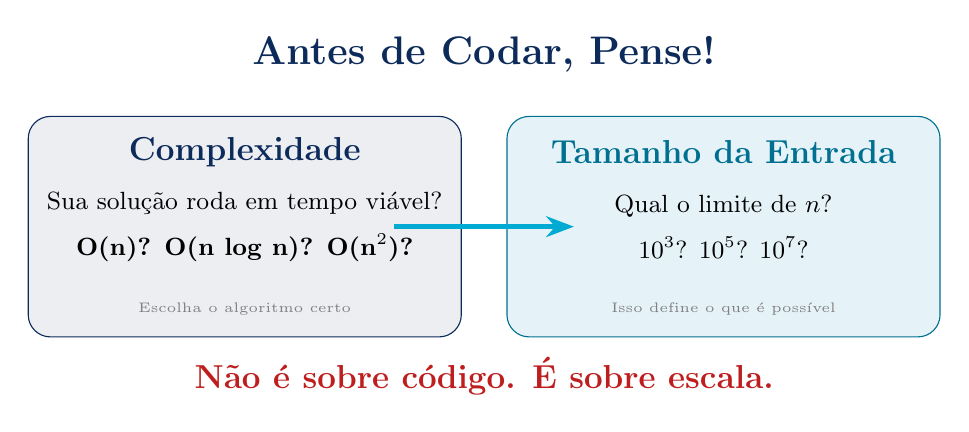
\begin{tikzpicture}[scale=0.95]

    % ── TÍTULO CENTRAL ─────────────────────────────────────
    \node[font=\bfseries\Large,gemaBlue] at (6,5.5){
      Antes de Codar, Pense!
    };

    % ── BLOCO COMPLEXIDADE ────────────────────────────────
    \node[draw=gemaBlue,fill=gemaBlue!8,rounded corners=8pt,
          minimum width=5.5cm,minimum height=2.8cm] (comp) at (2.8,3.2){};

    \node[font=\bfseries\large,gemaBlue] at (2.8,4.2){
      Complexidade
    };

    \node[font=\small,align=center] at (2.8,3.2){
      Sua solução roda em tempo viável?\\[0.2cm]
      \textbf{O(n)? O(n log n)? O(n$^2$)?}
    };

    \node[font=\tiny,gray] at (2.8,2.1){
      Escolha o algoritmo certo
    };

    % ── BLOCO ENTRADA ─────────────────────────────────────
    \node[draw=queueColor!80!black,fill=queueColor!10,rounded corners=8pt,
          minimum width=5.5cm,minimum height=2.8cm] (input) at (9.2,3.2){};

    \node[font=\bfseries\large,queueColor!80!black] at (9.2,4.2){
      Tamanho da Entrada
    };

    \node[font=\small,align=center] at (9.2,3.2){
      Qual o limite de $n$?\\[0.2cm]
      $10^3$? $10^5$? $10^7$?
    };

    \node[font=\tiny,gray] at (9.2,2.1){
      Isso define o que é possível
    };

    % ── SETA CENTRAL ──────────────────────────────────────
    \draw[-{Stealth[length=10pt]},line width=2pt,gemaCyan]
      (4.8,3.2) -- (7.2,3.2);

    % ── FRASE DE IMPACTO ──────────────────────────────────
    \node[font=\bfseries\large,gemaRed] at (6,1.2){
      Não é sobre código. É sobre escala.
    };

  \end{tikzpicture}
  \end{adjustbox}
\end{frame}
% =============================================================
%  DIVISOR REVISAO
% =============================================================
{
\setbeamertemplate{footline}{}
\begin{frame}[noframenumbering]
  \centering\vspace{1.0cm}
  {\fontsize{30}{36}\selectfont\bfseries\color{gemaBlue} Revisão}\par
  \vspace{0.25cm}
  {\Large\color{gemaCyan}\bfseries Stack vs.\ Queue}\par
  \vspace{0.15cm}
  {\color{gray}\small LIFO $\times$ FIFO}
\end{frame}
}

% ─────────────────────────────────────────────────────────────
%  STACK VS QUEUE — VISUAL
% ─────────────────────────────────────────────────────────────
\begin{frame}{Stack vs.\ Queue: Comparacão Visual}
  \centering
  \begin{adjustbox}{max totalsize={0.98\textwidth}{0.80\textheight},center}
  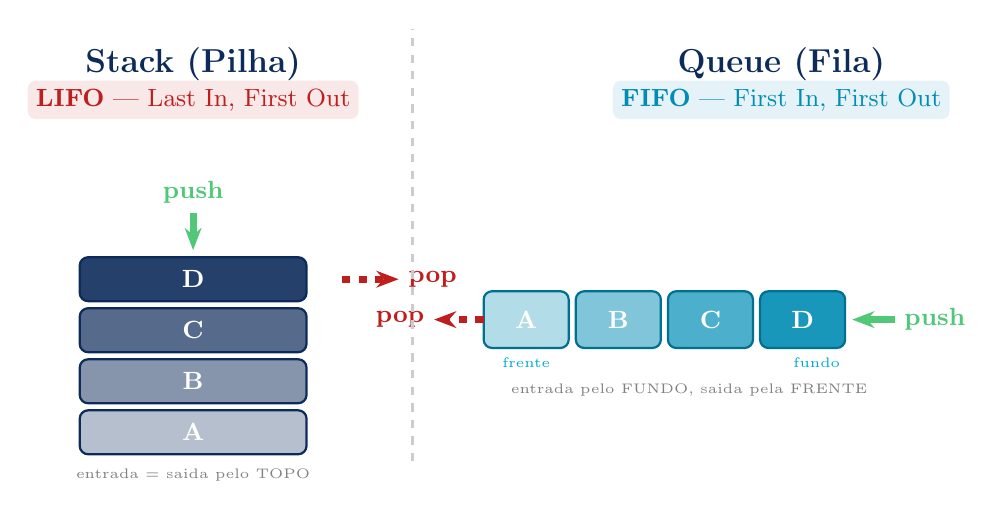
\begin{tikzpicture}[scale=0.90]

    % ── STACK ──────────────────────────────────────────────
    \node[font=\bfseries\large,gemaBlue] at (2.2,5.5){Stack (Pilha)};
    \node[font=\small,gemaRed,fill=gemaRed!10,rounded corners=3pt,inner sep=3pt]
      at (2.2,5.0){\textbf{LIFO} --- Last In, First Out};
    \foreach \val/\shade/\y in {A/30/0, B/50/0.72, C/70/1.44, D/90/2.16}{
      \draw[fill=gemaBlue!\shade,draw=gemaBlue,rounded corners=3pt,line width=0.8pt]
        (0.6,\y) rectangle (3.8,\y+0.62)
        node[midway,white,font=\bfseries\small]{\val};
    }
    \draw[-{Stealth[length=8pt]},codeGreen,line width=2.5pt](2.2,3.4)--(2.2,2.88);
    \node[above,codeGreen,font=\bfseries\small] at (2.2,3.4){push};
    \draw[-{Stealth[length=8pt]},gemaRed,line width=2.5pt,dashed](4.3,2.47)--(5.1,2.47);
    \node[right,gemaRed,font=\bfseries\small] at (5.1,2.47){pop};
    \node[font=\tiny,gray] at (2.2,-0.3){entrada = saida pelo TOPO};
    % \node[font=\footnotesize,gemaBlue,fill=gemaBlue!6,rounded corners=3pt,
    %       inner sep=3pt,align=center] at (2.2,-0.9){ \\ Ctrl+Z \\ Chamadas};

    % ── QUEUE ──────────────────────────────────────────────
    \node[font=\bfseries\large,gemaBlue] at (10.5,5.5){Queue (Fila)};
    \node[font=\small,queueColor,fill=queueColor!10,rounded corners=3pt,inner sep=3pt]
      at (10.5,5.0){\textbf{FIFO} --- First In, First Out};
    \foreach \val/\shade/\x in {A/30/6.3, B/50/7.6, C/70/8.9, D/90/10.2}{
      \draw[fill=queueColor!\shade,draw=queueColor!80!black,rounded corners=3pt,line width=0.8pt]
        (\x,1.5) rectangle (\x+1.2,2.3)
        node[midway,white,font=\bfseries\small]{\val};
    }
    \draw[-{Stealth[length=8pt]},codeGreen,line width=2.5pt](12.1,1.9)--(11.5,1.9);
    \node[right,codeGreen,font=\bfseries\small] at (12.1,1.9){push};
    \draw[-{Stealth[length=8pt]},gemaRed,line width=2.5pt,dashed](6.3,1.9)--(5.6,1.9);
    \node[left,gemaRed,font=\bfseries\small] at (5.6,1.9){pop};
    \node[font=\tiny,gemaCyan,below] at (6.9,1.5){frente};
    \node[font=\tiny,gemaCyan,below] at (11.0,1.5){fundo};
    \node[font=\tiny,gray] at (9.2,0.9){entrada pelo FUNDO, saida pela FRENTE};
    % \node[font=\footnotesize,queueColor!80!black,fill=queueColor!6,
    %       rounded corners=3pt,inner sep=3pt,align=center] at (10.5,-0.9)
    %   {Fila de banco \\ Impressora \\ BFS};

    % separador
    \draw[gray!40,dashed,line width=1pt](5.3,-0.1)--(5.3,6.0);

  \end{tikzpicture}
  \end{adjustbox}
\end{frame}

% =============================================================
%  DIVISOR PARTE 1
% =============================================================
{
\setbeamertemplate{footline}{}
\begin{frame}[noframenumbering]
  \centering\vspace{1.2cm}
  {\fontsize{38}{46}\selectfont\bfseries\color{gemaBlue} 1}\par
  \vspace{0.25cm}
  {\Large\color{gemaCyan}\bfseries Queue (Fila)}\par
  \vspace{0.15cm}
  {\color{gray}\small FIFO $\cdot$ Operacoes $\cdot$ Implementação $\cdot$ BFS}
\end{frame}
}

% ─────────────────────────────────────────────────────────────
%  CONCEITO DE FILA
% ─────────────────────────────────────────────────────────────
\begin{frame}{O que é uma Queue (Fila)?}
  \begin{columns}[c]
    \column{0.50\textwidth}
      \begin{tcolorbox}[caixaAzul,title={Definição}]
        \small Uma \textbf{fila} e uma estrutura linear onde o
        \textbf{primeiro elemento inserido} e o
        \textbf{primeiro a ser removido}.
      \end{tcolorbox}
      \vspace{0.12cm}
      \begin{tcolorbox}[caixaLaranja,title={FIFO}]
        \small\textbf{F}irst \textbf{I}n, \textbf{F}irst \textbf{O}ut\\[2pt]
        Entrada pelo \textbf{fundo}, saida pela \textbf{frente}.
      \end{tcolorbox}
      \vspace{0.12cm}
      \textbf{\small Analogias:}
      \begin{itemize}\footnotesize
        \item Fila de banco ou supermercado
        \item Fila de impressora
        \item Passageiros embarcando no onibus
        \item Pacotes de rede aguardando envio
      \end{itemize}
    \column{0.48\textwidth}
      \centering
      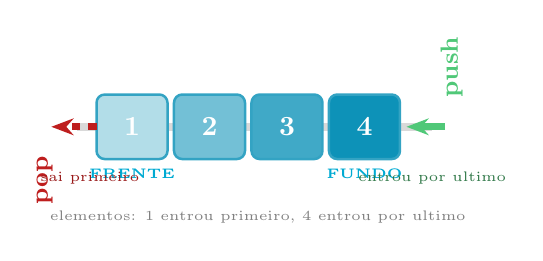
\begin{tikzpicture}[scale=0.82]
        \draw[gray!30,line width=3pt] (0,1.0)--(5.5,1.0);
        \foreach \val/\shade/\x in {1/30/0.3, 2/55/1.5, 3/75/2.7, 4/95/3.9}{
          \draw[fill=queueColor!\shade,draw=queueColor!80,rounded corners=3pt,line width=0.9pt]
            (\x,0.5) rectangle (\x+1.1,1.5)
            node[midway,white,font=\bfseries]{\val};
        }
        \draw[-{Stealth[length=8pt]},codeGreen,line width=2.5pt](5.7,1.0)--(5.1,1.0);
        \node[right,codeGreen,font=\bfseries\small,rotate=90] at (5.8,1.3){push};
        \draw[-{Stealth[length=8pt]},gemaRed,line width=2.5pt,dashed](0.3,1.0)--(-0.4,1.0);
        \node[left,gemaRed,font=\bfseries\small,rotate=90] at (-0.5,0.7){pop};
        \node[gemaCyan,font=\tiny\bfseries,below] at (0.85,0.5){FRENTE};
        \node[gemaCyan,font=\tiny\bfseries,below] at (4.45,0.5){FUNDO};
        \node[codeGreen!60!black,font=\tiny] at (5.5,0.2){entrou por ultimo};
        \node[gemaRed!80!black,font=\tiny] at (0.2,0.2){sai primeiro};
        \node[font=\tiny,gray,below] at (2.8,-0.15)
          {elementos: 1 entrou primeiro, 4 entrou por ultimo};
      \end{tikzpicture}
      \vspace{0.15cm}
      \begin{tcolorbox}[caixaVerde,title={Chave}]
        \footnotesize
        Quem chegou \textbf{primeiro} na fila
        é o \textbf{primeiro} a ser atendido.
      \end{tcolorbox}
  \end{columns}
\end{frame}

% ─────────────────────────────────────────────────────────────
%  OPERAÇÕES
% ─────────────────────────────────────────────────────────────
\begin{frame}[shrink=2]{Operacoes da Queue}
  \begin{columns}[t]
    \column{0.31\textwidth}
      \begin{exampleblock}{push(x) / enqueue}
        \footnotesize
        Insere \texttt{x} no \textbf{fundo}.\\[3pt]
        \textbf{O(1)} sempre.\\[3pt]
        Nunca falha por si so.
      \end{exampleblock}
    \column{0.31\textwidth}
      \begin{alertblock}{pop() / dequeue}
        \footnotesize
        Remove a \textbf{frente}.\\[3pt]
        \textbf{O(1)}\\[3pt]
        \textcolor{gemaRed}{\textbf{CRASH se vazia!}}
      \end{alertblock}
    \column{0.31\textwidth}
      \begin{block}{front() / back()}
        \footnotesize
        Le a frente / o fundo\\sem remover.\\[3pt]
        \textbf{O(1)} ambos.\\
        \textcolor{gemaRed}{\textbf{CRASH se vazia!}}
      \end{block}
  \end{columns}
  \vspace{0.12cm}
  \begin{columns}[t]
    \column{0.31\textwidth}
      \begin{block}{empty()}
        \footnotesize
        \texttt{true} se vazia.\\[3pt]
        \textbf{Use SEMPRE antes}\\de \texttt{front()} e \texttt{pop()}.
      \end{block}
    \column{0.31\textwidth}
      \begin{block}{size()}
        \footnotesize
        Numero de elementos.\\[3pt]
        \textbf{O(1)}
      \end{block}
    \column{0.31\textwidth}
      \begin{tcolorbox}[caixaVerde,title={Dica de Prova}]
        \footnotesize
        Cheque \texttt{!q.empty()}\\
        antes de \texttt{front()}\\e \texttt{pop()}.
      \end{tcolorbox}
  \end{columns}
  \vspace{0.12cm}
  \begin{tcolorbox}[caixaAzul,title={Diferença critica: Queue vs Stack}]
    \centering\footnotesize
    \begin{tabular}{lll}
      \toprule
      & \textbf{Stack} & \textbf{Queue}\\
      \midrule
      Inserir & \texttt{push} $\to$ topo & \texttt{push} $\to$ fundo\\
      Remover & \texttt{pop} do topo & \texttt{pop} da frente\\
      Ler     & \texttt{top()} & \texttt{front()}\\
      \bottomrule
    \end{tabular}
  \end{tcolorbox}
\end{frame}

% ─────────────────────────────────────────────────────────────
%  QUEUE — PASSO A PASSO
% ─────────────────────────────────────────────────────────────
\begin{frame}{Queue --- Passo a Passo}
  \centering
  \begin{adjustbox}{max totalsize={0.97\textwidth}{0.80\textheight},center}
  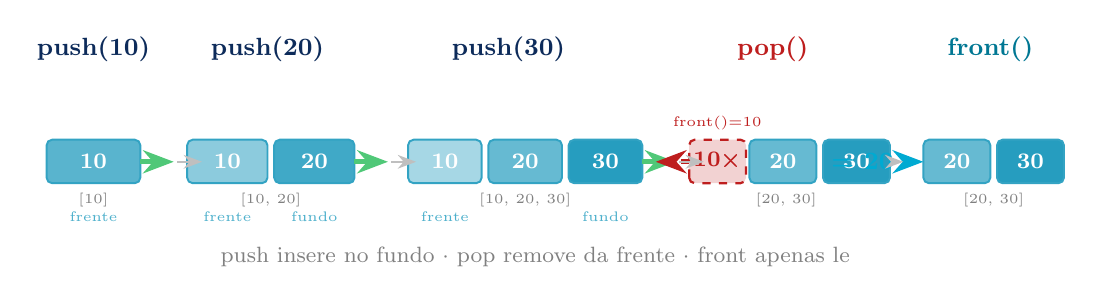
\begin{tikzpicture}[scale=0.85]

    % Estado 1: push(10)
    \node[font=\bfseries\small,gemaBlue] at (0.9,3.0){push(10)};
    \draw[fill=queueColor!65,draw=queueColor!80,rounded corners=2pt,line width=0.7pt]
      (0.2,1.0) rectangle (1.6,1.65) node[midway,white,font=\bfseries\footnotesize]{10};
    \draw[-{Stealth},codeGreen,line width=1.8pt](1.6,1.32)--(2.1,1.32);
    \node[font=\tiny,gray,below] at (0.9,1.0){[10]};
    \node[font=\tiny,queueColor!70,below] at (0.9,0.72){frente};

    % Estado 2: push(20)
    \node[font=\bfseries\small,gemaBlue] at (3.5,3.0){push(20)};
    \draw[fill=queueColor!45,draw=queueColor!80,rounded corners=2pt,line width=0.7pt]
      (2.3,1.0) rectangle (3.5,1.65) node[midway,white,font=\bfseries\footnotesize]{10};
    \draw[fill=queueColor!75,draw=queueColor!80,rounded corners=2pt,line width=0.7pt]
      (3.6,1.0) rectangle (4.8,1.65) node[midway,white,font=\bfseries\footnotesize]{20};
    \draw[-{Stealth},codeGreen,line width=1.8pt](4.8,1.32)--(5.3,1.32);
    \node[font=\tiny,gray,below] at (3.55,1.0){[10, 20]};
    \node[font=\tiny,queueColor!70,below] at (2.9,0.72){frente};
    \node[font=\tiny,queueColor!70,below] at (4.2,0.72){fundo};

    % Estado 3: push(30)
    \node[font=\bfseries\small,gemaBlue] at (7.1,3.0){push(30)};
    \draw[fill=queueColor!35,draw=queueColor!80,rounded corners=2pt,line width=0.7pt]
      (5.6,1.0) rectangle (6.7,1.65) node[midway,white,font=\bfseries\footnotesize]{10};
    \draw[fill=queueColor!60,draw=queueColor!80,rounded corners=2pt,line width=0.7pt]
      (6.8,1.0) rectangle (7.9,1.65) node[midway,white,font=\bfseries\footnotesize]{20};
    \draw[fill=queueColor!85,draw=queueColor!80,rounded corners=2pt,line width=0.7pt]
      (8.0,1.0) rectangle (9.1,1.65) node[midway,white,font=\bfseries\footnotesize]{30};
    \draw[-{Stealth},codeGreen,line width=1.8pt](9.1,1.32)--(9.6,1.32);
    \node[font=\tiny,gray,below] at (7.35,1.0){[10, 20, 30]};
    \node[font=\tiny,queueColor!70,below] at (6.15,0.72){frente};
    \node[font=\tiny,queueColor!70,below] at (8.55,0.72){fundo};

    % Estado 4: pop()
    \node[font=\bfseries\small,gemaRed] at (11.05,3.0){pop()};
    \draw[fill=gemaRed!20,draw=gemaRed,rounded corners=2pt,line width=0.8pt,dashed]
      (9.8,1.0) rectangle (10.65,1.65)
      node[midway,gemaRed,font=\bfseries\footnotesize]{10\texttimes};
    \draw[-{Stealth},gemaRed,line width=1.8pt,dashed](9.8,1.32)--(9.3,1.32);
    \draw[fill=queueColor!60,draw=queueColor!80,rounded corners=2pt,line width=0.7pt]
      (10.7,1.0) rectangle (11.7,1.65) node[midway,white,font=\bfseries\footnotesize]{20};
    \draw[fill=queueColor!85,draw=queueColor!80,rounded corners=2pt,line width=0.7pt]
      (11.8,1.0) rectangle (12.8,1.65) node[midway,white,font=\bfseries\footnotesize]{30};
    \node[font=\tiny,gray,below] at (11.25,1.0){[20, 30]};
    \node[font=\tiny,gemaRed,above] at (10.22,1.65){front()=10};

    % Estado 5: front()
    \node[font=\bfseries\small,gemaCyan!70!black] at (14.3,3.0){front()};
    \draw[fill=queueColor!60,draw=queueColor!80,rounded corners=2pt,line width=0.7pt]
      (13.3,1.0) rectangle (14.3,1.65) node[midway,white,font=\bfseries\footnotesize]{20};
    \draw[fill=queueColor!85,draw=queueColor!80,rounded corners=2pt,line width=0.7pt]
      (14.4,1.0) rectangle (15.4,1.65) node[midway,white,font=\bfseries\footnotesize]{30};
    \draw[-{Stealth},gemaCyan,line width=1.8pt](13.0,1.32)--(13.3,1.32);
    \node[left,gemaCyan,font=\bfseries\small] at (13.0,1.32){= 20};
    \node[font=\tiny,gray,below] at (14.35,1.0){[20, 30]};

    % setas de transição
    \foreach \x in {2.1,5.3,9.6}{
      \draw[-{Stealth},gray!50,line width=0.8pt](\x+0.05,1.32)--(\x+0.42,1.32);
    }
    \draw[-{Stealth},gray!50,line width=0.8pt](12.85,1.32)--(13.0,1.32);

    \node[font=\footnotesize,gray] at (7.5,-0.1)
      {push insere no fundo $\cdot$ pop remove da frente $\cdot$ front apenas le};

  \end{tikzpicture}
  \end{adjustbox}
\end{frame}

% ─────────────────────────────────────────────────────────────
%  IMPLEMENTAÇÃO STL — QUEUE
% ─────────────────────────────────────────────────────────────
\begin{frame}[fragile,shrink=3]{Implementação em C++ --- Queue}
  \begin{columns}[t]
    \column{0.59\textwidth}
      \begin{tcolorbox}[caixaCodigo]
        \begin{lstlisting}[style=cppstyle]
#include <bits/stdc++.h>
using namespace std;

int main() {
    queue<int> q;  // fila de inteiros

    q.push(10);    // insere no fundo: [10]
    q.push(20);    // insere no fundo: [10, 20]
    q.push(30);    // insere no fundo: [10, 20, 30]

    // SEMPRE verifica antes de acessar!
    cout << q.front() << "\n"; // 10 (frente)
    cout << q.back()  << "\n"; // 30 (fundo)

    q.pop();   // remove da frente -> [20, 30]
    cout << q.front() << "\n"; // 20
    cout << q.size()  << "\n"; // 2

    while (!q.empty()) {
        cout << q.front() << " "; // 20 30
        q.pop();
    }
    return 0;
}
        \end{lstlisting}
      \end{tcolorbox}
    \column{0.39\textwidth}
      \begin{tcolorbox}[caixaAzul,title={Resumo STL}]
        \footnotesize
        \begin{tabular}{@{}ll@{}}
          \texttt{push(x)}  & insere no fundo\\[2pt]
          \texttt{pop()}    & remove da frente\\[2pt]
          \texttt{front()}  & le a frente\\[2pt]
          \texttt{back()}   & le o fundo\\[2pt]
          \texttt{empty()}  & esta vazia?\\[2pt]
          \texttt{size()}   & quantos?\\
        \end{tabular}
      \end{tcolorbox}
      \vspace{0.1cm}
      \begin{tcolorbox}[caixaVermelho,title={Atenção}]
        \footnotesize
        \textbf{não existe} \texttt{top()} na queue!\\[2pt]
        Use \texttt{front()} para ler\\
        o primeiro elemento.\\[2pt]
        \texttt{pop()} remove\\
        \textbf{sem retornar} o valor.
      \end{tcolorbox}
      \vspace{0.1cm}
      \begin{tcolorbox}[caixaVerde,title={Tipos possiveis}]
        \footnotesize
        \texttt{queue<int>}\\
        \texttt{queue<long long>}\\
        \texttt{queue<string>}\\
        \texttt{queue<pair<int,int>>}
      \end{tcolorbox}
  \end{columns}
\end{frame}

% ─────────────────────────────────────────────────────────────
%  COMPLEXIDADE — QUEUE
% ─────────────────────────────────────────────────────────────
\begin{frame}{Complexidade da Queue}
  \begin{columns}[c]
    \column{0.50\textwidth}
      \begin{tcolorbox}[caixaAzul,title={Tabela de Complexidade}]
        \centering\footnotesize
        \begin{tabular}{lcc}
          \toprule
          \textbf{Operação} & \textbf{Tempo} & \textbf{Espaço}\\
          \midrule
          \texttt{push(x)}  & O(1) & O(1)\\
          \texttt{pop()}    & O(1) & O(1)\\
          \texttt{front()}  & O(1) & O(1)\\
          \texttt{back()}   & O(1) & O(1)\\
          \texttt{empty()}  & O(1) & O(1)\\
          \texttt{size()}   & O(1) & O(1)\\
          \midrule
          \textbf{Espaco total} & --- & O(n)\\
          \bottomrule
        \end{tabular}
      \end{tcolorbox}
      \vspace{0.1cm}
      \begin{tcolorbox}[caixaVerde,title={Por que tudo e O(1)?}]
        \small
        A STL usa um \textbf{deque} internamente,
        permitindo inserção e remoção eficiente
        em ambas as extremidades.
      \end{tcolorbox}
    \column{0.47\textwidth}
      \begin{tcolorbox}[caixaAmarelo,title={Stack vs Queue --- mesma eficiencia}]
        \footnotesize
        \begin{tabular}{lcc}
          \toprule
          & \textbf{Stack} & \textbf{Queue}\\
          \midrule
          push & O(1) & O(1)\\
          pop  & O(1) & O(1)\\
          peek & O(1) & O(1)\\
          \bottomrule
        \end{tabular}\\[5pt]
        A diferença é \textbf{comportamental}:\\
        LIFO vs FIFO.
      \end{tcolorbox}
      \vspace{0.1cm}
      \begin{tcolorbox}[caixaVermelho,title={Limitacoes da Queue}]
        \footnotesize
        A STL \textbf{não} permite:
        \begin{itemize}\footnotesize
          \item Acesso por indice (\texttt{q[i]})
          \item Iterar sem destruir a fila
          \item Pesquisa por valor
        \end{itemize}
        Se precisar: use \texttt{deque<T>}.
      \end{tcolorbox}
  \end{columns}
\end{frame}

% ─────────────────────────────────────────────────────────────
%  BFS — APLICAÇÃO
% ─────────────────────────────────────────────────────────────
\begin{frame}{Aplicação Classica --- BFS (Busca em Largura)}
  \begin{columns}[c]
    \column{0.48\textwidth}
      \begin{tcolorbox}[caixaAzul,title={O que é BFS?}]
        \small
        Explora um grafo \textbf{nível por nível}.
        A Queue garante que os nos sao
        visitados na ordem correta (FIFO).
      \end{tcolorbox}
      \vspace{0.1cm}
      \textbf{\small Algoritmo:}
      \begin{enumerate}\footnotesize
        \item Insere o nó inicial na queue
        \item Enquanto a queue não esta vazia:
        \begin{itemize}\footnotesize
          \item Retira o nó da frente
          \item Marca como visitado
          \item Insere vizinhos não visitados
        \end{itemize}
      \end{enumerate}
      \vspace{0.1cm}
      \begin{tcolorbox}[caixaAmarelo,title={Aplicacoes na OBI}]
        \footnotesize
        Menor caminho em labirinto\\
        Menor numero de movimentos\\
        Propagação em grade (``onda'')
      \end{tcolorbox}
    \column{0.50\textwidth}
      \centering
      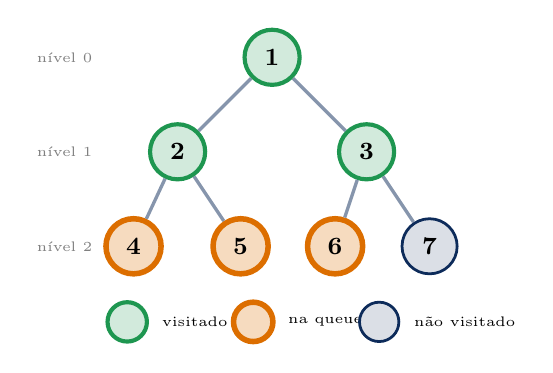
\begin{tikzpicture}[scale=0.80,
          no/.style={circle,draw=gemaBlue,fill=gemaBlue!15,
                     minimum size=7mm,font=\bfseries\small,line width=1pt},
          vis/.style={circle,draw=nodeGreen,fill=nodeGreen!20,
                      minimum size=7mm,font=\bfseries\small,line width=1.5pt},
          fron/.style={circle,draw=gemaOrange,fill=gemaOrange!25,
                       minimum size=7mm,font=\bfseries\small,line width=2pt},
        ]
        \node[vis]  (1) at (2.5,3.5){1};
        \node[vis]  (2) at (1.0,2.0){2};
        \node[vis]  (3) at (4.0,2.0){3};
        \node[fron] (4) at (0.3,0.5){4};
        \node[fron] (5) at (2.0,0.5){5};
        \node[fron] (6) at (3.5,0.5){6};
        \node[no]   (7) at (5.0,0.5){7};
        \foreach \a/\b in {1/2,1/3,2/4,2/5,3/6,3/7}{
          \draw[gemaBlue!50,line width=1.2pt](\a)--(\b);
        }
        \node[vis,minimum size=5mm] at (0.2,-0.7){};
        \node[font=\tiny,right] at (0.6,-0.7){visitado};
        \node[fron,minimum size=5mm] at (2.2,-0.7){};
        \node[font=\tiny,right] at (2.6,-0.7){na queue};
        \node[no,minimum size=5mm] at (4.2,-0.7){};
        \node[font=\tiny,right] at (4.6,-0.7){não visitado};
        \node[font=\tiny,gray,left] at (-0.2,3.5){nível 0};
        \node[font=\tiny,gray,left] at (-0.2,2.0){nível 1};
        \node[font=\tiny,gray,left] at (-0.2,0.5){nível 2};
      \end{tikzpicture}
      \vspace{0.05cm}
      \begin{tcolorbox}[caixaVerde,title={Estado atual}]
        \footnotesize
        Queue: \texttt{[4, 5, 6]}\\
        Visitados: \texttt{1, 2, 3}\\
        Stack (LIFO) faria DFS, não BFS!
      \end{tcolorbox}
  \end{columns}
\end{frame}

% ─────────────────────────────────────────────────────────────
%  BFS — CÓDIGO
% ─────────────────────────────────────────────────────────────
\begin{frame}[fragile,shrink=5]{BFS em Grafo --- Código Completo}
  \begin{columns}[t]
    \column{0.58\textwidth}
      \begin{tcolorbox}[caixaCodigo]
        \begin{lstlisting}[style=cppsmall]
#include <bits/stdc++.h>
using namespace std;

void bfs(int inicio, int N,
         vector<vector<int>>& adj) {

    vector<bool> visitado(N+1, false);
    vector<int>  dist(N+1, -1);
    queue<int> q;

    q.push(inicio);         // insere no inicial
    visitado[inicio] = true;
    dist[inicio] = 0;

    while (!q.empty()) {
        int v = q.front(); // pega a frente
        q.pop();           // remove da fila

        cout << "No " << v
             << " dist=" << dist[v] << "\n";

        for (int u : adj[v]) {
            if (!visitado[u]) {
                visitado[u] = true;
                dist[u] = dist[v] + 1;
                q.push(u); // insere no fundo
            }
        }
    }
}
        \end{lstlisting}
      \end{tcolorbox}
    \column{0.40\textwidth}
      \begin{tcolorbox}[caixaAzul,title={Por que Queue?}]
        \footnotesize
        Queue garante visita\\
        \textbf{nível por nível}.\\[3pt]
        Com Stack fariamos\\
        DFS, não BFS!
      \end{tcolorbox}
      \vspace{0.08cm}
      \begin{tcolorbox}[caixaVerde,title={Complexidade BFS}]
        \footnotesize
        \textbf{Tempo:} O(V + E)\\
        V = vértices, E = arestas\\[3pt]
        \textbf{Espaco:} O(V)\\[3pt]
        \textbf{Garante:} distância\\
        minima em grafos sem peso.
      \end{tcolorbox}
      \vspace{0.08cm}
      \begin{tcolorbox}[caixaAmarelo,title={Padrao de uso}]
        \footnotesize
        \texttt{q.push(inicio);}\\
        \texttt{while(!q.empty())\{}\\
        \texttt{\ \ v=q.front();}\\
        \texttt{\ \ q.pop();}\\
        \texttt{\ \ // processa v}\\
        \texttt{\}}
      \end{tcolorbox}
  \end{columns}
\end{frame}

% =============================================================
%  DIVISOR PARTE 2
% =============================================================
{
\setbeamertemplate{footline}{}
\begin{frame}[noframenumbering]
  \centering\vspace{1.2cm}
  {\fontsize{38}{46}\selectfont\bfseries\color{gemaBlue} 2}\par
  \vspace{0.25cm}
  {\Large\color{pqColor}\bfseries Fila de Prioridade}\par
  \vspace{0.15cm}
  {\color{gray}\small Heap $\cdot$ Max/Min $\cdot$ Dijkstra $\cdot$ Agendamento}
\end{frame}
}

% ─────────────────────────────────────────────────────────────
%  INTRODUÇÃO — PRIORITY QUEUE
% ─────────────────────────────────────────────────────────────
\begin{frame}{Introdução --- Fila de Prioridade}
  \begin{columns}[c]
    \column{0.50\textwidth}
      \begin{tcolorbox}[caixaRoxa,title={Problema com Queue simples}]
        \small
        E se precisarmos sempre atender o
        \textbf{elemento mais importante}
        independente da ordem de chegada?
      \end{tcolorbox}
      \vspace{0.1cm}
      \begin{tcolorbox}[caixaAzul,title={Solução: Priority Queue}]
        \small
        Uma \textbf{fila de prioridade} associa
        uma \textbf{prioridade} a cada elemento.
        O de \textbf{maior (ou menor) prioridade}
        e sempre o primeiro a sair.
      \end{tcolorbox}
      \vspace{0.1cm}
      \textbf{\small Analogias:}
      \begin{itemize}\footnotesize
        \item Fila de emergencia no hospital
        \item Servidor processando tarefa urgente
        \item Dijkstra: expande menor distância
      \end{itemize}
    \column{0.48\textwidth}
      \centering
      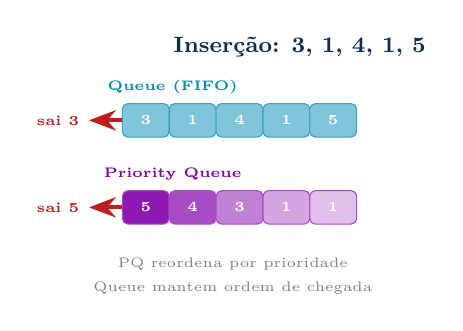
\begin{tikzpicture}[scale=0.85]
        \node[font=\bfseries\footnotesize,gemaBlue] at (2.5,4.0)
          {Inserção: 3, 1, 4, 1, 5};

        % Queue normal
        \node[font=\tiny\bfseries,queueColor] at (0.6,3.4){Queue (FIFO)};
        \foreach \val/\x in {3/0.0, 1/0.7, 4/1.4, 1/2.1, 5/2.8}{
          \draw[fill=queueColor!50,draw=queueColor!80,rounded corners=2pt]
            (\x-0.15,2.65) rectangle (\x+0.55,3.15)
            node[midway,white,font=\tiny\bfseries]{\val};
        }
        \draw[-{Stealth},gemaRed,line width=1.5pt](-0.15,2.9)--(-0.65,2.9);
        \node[left,gemaRed,font=\tiny\bfseries] at (-0.65,2.9){sai 3};

        % Priority Queue
        \node[font=\tiny\bfseries,pqColor] at (0.6,2.1){Priority Queue};
        \foreach \val/\shade/\x in {5/90/0.0, 4/70/0.7, 3/50/1.4, 1/35/2.1, 1/25/2.8}{
          \draw[fill=pqColor!\shade,draw=pqColor!70,rounded corners=2pt]
            (\x-0.15,1.35) rectangle (\x+0.55,1.85)
            node[midway,white,font=\tiny\bfseries]{\val};
        }
        \draw[-{Stealth},gemaRed,line width=1.5pt](-0.15,1.6)--(-0.65,1.6);
        \node[left,gemaRed,font=\tiny\bfseries] at (-0.65,1.6){sai 5};

        \node[font=\tiny,gray] at (1.5,0.75){PQ reordena por prioridade};
        \node[font=\tiny,gray] at (1.5,0.4){Queue mantem ordem de chegada};
      \end{tikzpicture}
  \end{columns}
\end{frame}

% ─────────────────────────────────────────────────────────────
%  HEAP — ESTRUTURA INTERNA
% ─────────────────────────────────────────────────────────────
\begin{frame}{Heap --- Estrutura Interna}
  \begin{columns}[c]
    \column{0.46\textwidth}
      \begin{tcolorbox}[caixaAzul,title={O que é um Heap?}]
        \small
        Arvore binaria quase completa onde cada
        no e \textbf{maior (max-heap)} ou
        \textbf{menor (min-heap)} que seus filhos.
        A \textbf{raiz} e sempre o max ou min.
      \end{tcolorbox}
      \vspace{0.1cm}
      \begin{tcolorbox}[caixaVermelho,title={Max-Heap --- padrao STL}]
        \footnotesize Raiz = maior elemento.\\
        \texttt{priority\_queue<int>}
      \end{tcolorbox}
      \vspace{0.1cm}
      \begin{tcolorbox}[caixaVerde,title={Min-Heap}]
        \footnotesize Raiz = menor elemento.\\
        \texttt{priority\_queue<int,vector<int>,}\\
        \texttt{greater<int>>}
      \end{tcolorbox}
      \vspace{0.1cm}
      \begin{tcolorbox}[caixaAmarelo,title={Operacoes}]
        \footnotesize
        \texttt{push}: O(log n) ---
        \texttt{pop}: O(log n) ---
        \texttt{top}: O(1)
      \end{tcolorbox}
    \column{0.52\textwidth}
      \centering
      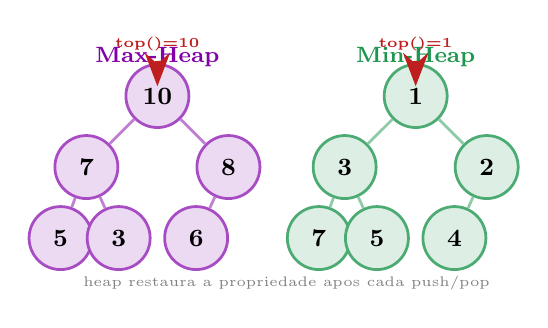
\begin{tikzpicture}[scale=0.82,
          maxno/.style={circle,draw=pqColor!70,fill=pqColor!15,
                        minimum size=8mm,font=\bfseries\small,line width=1pt},
          minno/.style={circle,draw=nodeGreen!80,fill=nodeGreen!15,
                        minimum size=8mm,font=\bfseries\small,line width=1pt},
        ]
        % MAX-HEAP
        \node[font=\bfseries\footnotesize,pqColor] at (1.5,4.3){Max-Heap};
        \node[maxno](r)  at (1.5,3.7){10};
        \node[maxno](l)  at (0.4,2.6){7};
        \node[maxno](rr) at (2.6,2.6){8};
        \node[maxno](ll) at (0.0,1.5){5};
        \node[maxno](lr) at (0.9,1.5){3};
        \node[maxno](rl) at (2.1,1.5){6};
        \draw[pqColor!50,line width=1pt](r)--(l)(r)--(rr)(l)--(ll)(l)--(lr)(rr)--(rl);
        \draw[-{Stealth},gemaRed,line width=2pt](1.5,4.25)--(1.5,3.85);
        \node[above,gemaRed,font=\tiny\bfseries] at (1.5,4.25){top()=10};

        % MIN-HEAP
        \node[font=\bfseries\footnotesize,nodeGreen] at (5.5,4.3){Min-Heap};
        \node[minno](r2)  at (5.5,3.7){1};
        \node[minno](l2)  at (4.4,2.6){3};
        \node[minno](rr2) at (6.6,2.6){2};
        \node[minno](ll2) at (4.0,1.5){7};
        \node[minno](lr2) at (4.9,1.5){5};
        \node[minno](rl2) at (6.1,1.5){4};
        \draw[nodeGreen!50,line width=1pt](r2)--(l2)(r2)--(rr2)(l2)--(ll2)(l2)--(lr2)(rr2)--(rl2);
        \draw[-{Stealth},gemaRed,line width=2pt](5.5,4.25)--(5.5,3.85);
        \node[above,gemaRed,font=\tiny\bfseries] at (5.5,4.25){top()=1};

        \node[font=\tiny,gray] at (3.5,0.8)
          {heap restaura a propriedade apos cada push/pop};
      \end{tikzpicture}
  \end{columns}
\end{frame}

% ─────────────────────────────────────────────────────────────
%  IMPLEMENTAÇÃO — PRIORITY QUEUE
% ─────────────────────────────────────────────────────────────
\begin{frame}[fragile,shrink=3]{Implementação em C++ --- Priority Queue}
  \begin{columns}[t]
    \column{0.59\textwidth}
      \begin{tcolorbox}[caixaCodigo]
        \begin{lstlisting}[style=cppstyle]
#include <bits/stdc++.h>
using namespace std;

int main() {
    // MAX-HEAP (padrao): maior no topo
    priority_queue<int> maxpq;

    maxpq.push(3);
    maxpq.push(1);
    maxpq.push(4);
    maxpq.push(1);
    maxpq.push(5);

    cout << maxpq.top() << "\n"; // 5 (maior)
    maxpq.pop();
    cout << maxpq.top() << "\n"; // 4

    // MIN-HEAP: menor no topo
    priority_queue<int,
        vector<int>,
        greater<int>> minpq;

    minpq.push(3);
    minpq.push(1);
    minpq.push(4);

    cout << minpq.top() << "\n"; // 1 (menor)
    return 0;
}
        \end{lstlisting}
      \end{tcolorbox}
    \column{0.39\textwidth}
      \begin{tcolorbox}[caixaRoxa,title={Operacoes PQ}]
        \footnotesize
        \begin{tabular}{@{}ll@{}}
          \texttt{push(x)}  & insere\\[2pt]
          \texttt{pop()}    & remove topo\\[2pt]
          \texttt{top()}    & le o topo\\[2pt]
          \texttt{empty()}  & esta vazia?\\[2pt]
          \texttt{size()}   & quantos?\\
        \end{tabular}
      \end{tcolorbox}
      \vspace{0.08cm}
      \begin{tcolorbox}[caixaVermelho,title={Atenção}]
        \footnotesize
        \textbf{não existe} \texttt{front()}!\\[2pt]
        Use \texttt{top()} para ver\\
        o elemento prioritario.\\[2pt]
        \texttt{pop()} remove sem\\retornar o valor.
      \end{tcolorbox}
      \vspace{0.08cm}
      \begin{tcolorbox}[caixaVerde,title={Min-heap rapido}]
        \footnotesize
        Usando max-heap:\\
        \texttt{push(-x)} e depois\\
        \texttt{-top()} para ler.\\[2pt]
        Util em provas rapidas.
      \end{tcolorbox}
  \end{columns}
\end{frame}

% ─────────────────────────────────────────────────────────────
%  PQ COM PARES — DIJKSTRA
% ─────────────────────────────────────────────────────────────
\begin{frame}[fragile,shrink=3]{Priority Queue com Pares --- Padrao Dijkstra}
  \begin{tcolorbox}[caixaAmarelo,title={Por que usar pares?}]
    \footnotesize
    Em Dijkstra precisamos armazenar \textbf{(custo, no)}.
    O par e comparado pelo primeiro elemento automaticamente.
  \end{tcolorbox}
  \vspace{0.06cm}
  \begin{columns}[t]
    \column{0.57\textwidth}
      \begin{tcolorbox}[caixaCodigo]
        \begin{lstlisting}[style=cppsmall]
#include <bits/stdc++.h>
using namespace std;
typedef pair<int,int> pii;

int main(){
    // Min-heap de pares {custo, no}
    priority_queue<pii,
        vector<pii>,
        greater<pii>> pq;

    pq.push({10, 1}); // custo 10, no 1
    pq.push({3,  2}); // custo 3,  no 2
    pq.push({7,  3}); // custo 7,  no 3

    // sai o de MENOR custo primeiro
    while (!pq.empty()) {
        auto [custo, no] = pq.top();
        pq.pop();
        cout << "no=" << no
             << " custo=" << custo << "\n";
    }
    // Saida:
    //   no=2 custo=3
    //   no=3 custo=7
    //   no=1 custo=10
}
        \end{lstlisting}
      \end{tcolorbox}
    \column{0.41\textwidth}
      \begin{tcolorbox}[caixaAzul,title={Declaracoes comuns}]
        \footnotesize
        \textbf{Max-heap int:}\\
        \texttt{priority\_queue<int>}\\[4pt]
        \textbf{Min-heap int:}\\
        \texttt{priority\_queue<int,}\\
        \texttt{vector<int>,}\\
        \texttt{greater<int>>}\\[4pt]
        \textbf{Min-heap pares:}\\
        \texttt{priority\_queue<pii,}\\
        \texttt{vector<pii>,}\\
        \texttt{greater<pii>>}\\[4pt]
        \textbf{typedef:}\\
        \texttt{typedef pair<int,int> pii;}
      \end{tcolorbox}
      \vspace{0.08cm}
      \begin{tcolorbox}[caixaVerde,title={Comparação de pares}]
        \footnotesize
        Compara pelo \textbf{1o elemento}.\\
        Empate: compara o \textbf{2o}.\\[3pt]
        Dijkstra: \texttt{\{distância, no\}}
      \end{tcolorbox}
  \end{columns}
\end{frame}

% ─────────────────────────────────────────────────────────────
%  COMPLEXIDADE — PRIORITY QUEUE
% ─────────────────────────────────────────────────────────────
\begin{frame}{Complexidade da Priority Queue}
  \begin{columns}[c]
    \column{0.50\textwidth}
      \begin{tcolorbox}[caixaRoxa,title={Tabela de Complexidade}]
        \centering\footnotesize
        \begin{tabular}{lcc}
          \toprule
          \textbf{Operação} & \textbf{Tempo} & \textbf{Por que?}\\
          \midrule
          \texttt{push(x)}  & O(log n) & rebalanceia heap\\
          \texttt{pop()}    & O(log n) & rebalanceia heap\\
          \texttt{top()}    & O(1)     & raiz do heap\\
          \texttt{empty()}  & O(1)     & verifica tamanho\\
          \texttt{size()}   & O(1)     & contador interno\\
          \midrule
          Espaco total      & ---      & O(n)\\
          \bottomrule
        \end{tabular}
      \end{tcolorbox}
      \vspace{0.1cm}
      \begin{tcolorbox}[caixaVerde,title={Intuição do O(log n)}]
        \small
        O heap e uma arvore de altura $\log n$.
        Apos push ou pop, o elemento ``sobe''
        ou ``desce'' ate restaurar a propriedade.
        No maximo $\log n$ trocas.
      \end{tcolorbox}
    \column{0.47\textwidth}
      \begin{tcolorbox}[caixaAmarelo,title={Comparação geral}]
        \footnotesize
        \begin{tabular}{lccc}
          \toprule
          & \textbf{Queue} & \textbf{Stack} & \textbf{PQ}\\
          \midrule
          push & O(1) & O(1) & O(log n)\\
          pop  & O(1) & O(1) & O(log n)\\
          peek & O(1) & O(1) & O(1)\\
          \midrule
          ordem & FIFO & LIFO & prioridade\\
          \bottomrule
        \end{tabular}
      \end{tcolorbox}
      \vspace{0.1cm}
      \begin{tcolorbox}[caixaVermelho,title={O(log n) e rapido!}]
        \small
        Para $n = 10^6$:\\
        $\log_2(10^6) \approx 20$ trocas.\\[3pt]
        Processar $10^6$ elementos:\\
        $\approx 2{\times}10^7$ operacoes.\\
        \textbf{Muito rapido na pratica!}
      \end{tcolorbox}
  \end{columns}
\end{frame}

% ─────────────────────────────────────────────────────────────
%  DIJKSTRA — CÓDIGO
% ─────────────────────────────────────────────────────────────
\begin{frame}[fragile,shrink=5]{Aplicação Classica --- Dijkstra}
  \begin{columns}[t]
    \column{0.57\textwidth}
      \begin{tcolorbox}[caixaCodigo]
        \begin{lstlisting}[style=cppsmall]
#include <bits/stdc++.h>
using namespace std;
typedef pair<int,int> pii;
const int INF = 1e9;

vector<int> dijkstra(int inicio, int N,
    vector<vector<pii>>& adj) {

    vector<int> dist(N+1, INF);
    // min-heap: {distância, no}
    priority_queue<pii,vector<pii>,
                   greater<pii>> pq;

    dist[inicio] = 0;
    pq.push({0, inicio});

    while (!pq.empty()) {
        auto [d, v] = pq.top(); pq.pop();
        // descarta entradas desatualizadas
        if (d > dist[v]) continue;
        for (auto [peso, u] : adj[v]) {
            if (dist[v]+peso < dist[u]) {
                dist[u] = dist[v]+peso;
                pq.push({dist[u], u});
            }
        }
    }
    return dist;
}
        \end{lstlisting}
      \end{tcolorbox}
    \column{0.41\textwidth}
      \begin{tcolorbox}[caixaAzul,title={Por que PQ em Dijkstra?}]
        \footnotesize
        Sempre expandimos o no com
        a \textbf{menor distância}.\\[3pt]
        PQ (min-heap) acha em O(1).\\[3pt]
        Sem PQ: O($V^2$)\\
        Com PQ: O((V+E)log V)
      \end{tcolorbox}
      \vspace{0.08cm}
      \begin{tcolorbox}[caixaVerde,title={Grafo de exemplo}]
        \centering\footnotesize
        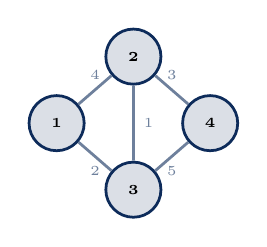
\begin{tikzpicture}[scale=0.65,
          no/.style={circle,draw=gemaBlue,fill=gemaBlue!15,
                     minimum size=7mm,font=\bfseries\tiny,line width=1pt}]
          \node[no](1) at (0,1.5){1};
          \node[no](2) at (1.5,2.8){2};
          \node[no](3) at (1.5,0.2){3};
          \node[no](4) at (3.0,1.5){4};
          \draw[gemaBlue!60,line width=1pt]
            (1)--(2) node[midway,above,font=\tiny]{4}
            (1)--(3) node[midway,below,font=\tiny]{2}
            (2)--(4) node[midway,above,font=\tiny]{3}
            (3)--(4) node[midway,below,font=\tiny]{5}
            (2)--(3) node[midway,right,font=\tiny]{1};
        \end{tikzpicture}\\[2pt]
        \texttt{dist=[0,4,2,6]}\\
        Caminho: 1$\to$3$\to$2$\to$4
      \end{tcolorbox}
      \vspace{0.08cm}
      \begin{tcolorbox}[caixaVermelho,title={Cuidado}]
        \footnotesize
        PQ pode ter entradas\\
        desatualizadas. Sempre:\\
        \texttt{if(d>dist[v]) continue;}
      \end{tcolorbox}
  \end{columns}
\end{frame}

% ─────────────────────────────────────────────────────────────
%  COMPARAÇÃO FINAL
% ─────────────────────────────────────────────────────────────
\begin{frame}{Queue vs.\ Priority Queue --- Quando Usar?}
  \begin{tcolorbox}[caixaAzul,title={Tabela Comparativa}]
    \centering\footnotesize
    \begin{tabular}{lll}
      \toprule
      \textbf{Criterio} & \textbf{Queue} & \textbf{Priority Queue}\\
      \midrule
      Ordem de saida & Chegada (FIFO) & Prioridade (maior/menor)\\
      push / pop     & O(1) & O(log n)\\
      peek           & O(1) --- \texttt{front()} & O(1) --- \texttt{top()}\\
      Algoritmo      & BFS, simulacoes & Dijkstra, Prim, A*\\
      Pergunta-chave & ``Chegou primeiro?'' & ``E mais importante?''\\
      \bottomrule
    \end{tabular}
  \end{tcolorbox}
  \vspace{0.1cm}
  \begin{columns}[t]
    \column{0.47\textwidth}
      \begin{tcolorbox}[caixaLaranja,title={Use Queue quando...}]
        \begin{itemize}\footnotesize
          \item A ordem de chegada importa
          \item Fazer BFS em grafo/grade
          \item Simular uma fila real
          \item Processar eventos em sequencia
        \end{itemize}
      \end{tcolorbox}
    \column{0.50\textwidth}
      \begin{tcolorbox}[caixaRoxa,title={Use Priority Queue quando...}]
        \begin{itemize}\footnotesize
          \item Precisa do maior/menor elemento rapido
          \item Implementar Dijkstra, Prim, A*
          \item Agendamento por urgência
          \item Mesclar listas ordenadas
        \end{itemize}
      \end{tcolorbox}
  \end{columns}
\end{frame}

% ─────────────────────────────────────────────────────────────
%  EXERCÍCIO PRÁTICO
% ─────────────────────────────────────────────────────────────
\begin{frame}[fragile,shrink=3]{Exercício Prático}
  \begin{tcolorbox}[caixaRoxa,title={Problema: Hospital de Campanha}]
    \footnotesize
    Um hospital recebe $Q$ eventos: \texttt{E g} (chega paciente com gravidade g)
    ou \texttt{A} (atende o mais grave). Imprima a gravidade atendida ou \texttt{-1} se vazia.\\[2pt]
    \textbf{Entrada:} \texttt{5 | E 3 | E 7 | E 1 | A | A}
    \quad\textbf{Saída:} \texttt{7\ \ 3}
  \end{tcolorbox}
  \vspace{0.06cm}
  \begin{columns}[t]
    \column{0.6\textwidth}
      \begin{tcolorbox}[caixaCodigo]
        \begin{lstlisting}[style=cppsmall]
#include <bits/stdc++.h>
using namespace std;

int main(){
    int Q; cin >> Q;
    priority_queue<int> pq; // max-heap

    while(Q--){
        char op; cin >> op;
        if(op == 'E'){
            int g; cin >> g;
            pq.push(g);      // novo paciente
        } else {
            if(pq.empty())
                cout << -1 << "\n";
            else {
                cout << pq.top() << "\n";
                pq.pop(); // atende o mais grave
            }
        }
    }
    return 0;
}
        \end{lstlisting}
      \end{tcolorbox}
    \column{0.46\textwidth}
      \begin{tcolorbox}[caixaAmarelo,title={Estrategia}]
        \footnotesize
        \textbf{1. Identificar a estrutura:}\\
        Preciso do \textbf{maior} rapidamente\\
        $\to$ Max-Heap!\\[4pt]
        \textbf{2. Modelar:}\\
        Evento E $\to$ \texttt{push}\\
        Evento A $\to$ \texttt{top} + \texttt{pop}\\[4pt]
        \textbf{3. Borda:}\\
        Fila vazia ao atender $\to$ \texttt{-1}\\[4pt]
        \textbf{Complexidade:} O(Q log Q)
      \end{tcolorbox}
      \vspace{0.08cm}
      \begin{tcolorbox}[caixaVerde,title={Variação com Queue}]
        \footnotesize
        Se o problema dissesse ``por\\
        ordem de chegada'' $\to$\\
        use \texttt{queue} com\\
        \texttt{front()} no lugar de \texttt{top()}.
      \end{tcolorbox}
  \end{columns}
\end{frame}

% ─────────────────────────────────────────────────────────────
%  COMO IDENTIFICAR NA PROVA
% ─────────────────────────────────────────────────────────────
\begin{frame}{Como Identificar na Prova?}
  \begin{columns}[t]
    \column{0.47\textwidth}
      \begin{block}{Palavras-chave para Queue}
        \begin{itemize}\footnotesize
          \item ``menor caminho em passos'' (BFS)
          \item ``nível a nível'', ``onda''
          \item ``fila de processamento''
          \item ``propaga para vizinhos''
          \item ``labirinto'', ``grade'', ``distância minima''
        \end{itemize}
      \end{block}
      \vspace{0.1cm}
      \begin{tcolorbox}[caixaLaranja,title={Sinal: use Queue}]
        \footnotesize
        Grafo/grade \textbf{sem pesos}\\e menor distância.
      \end{tcolorbox}
    \column{0.50\textwidth}
      \begin{block}{Palavras-chave para Priority Queue}
        \begin{itemize}\footnotesize
          \item ``maior prioridade'', ``mais urgente''
          \item ``menor custo'' (com pesos)
          \item ``$k$-esimo maior/menor''
          \item ``Dijkstra'', ``Prim'', ``A*''
          \item ``agendamento'', ``escalonamento''
        \end{itemize}
      \end{block}
      \vspace{0.1cm}
      \begin{tcolorbox}[caixaRoxa,title={Sinal: use Priority Queue}]
        \footnotesize
        Grafo com \textbf{pesos} e\\menor caminho, ou max/min rapido.
      \end{tcolorbox}
  \end{columns}
  \vspace{0.1cm}
  \begin{tcolorbox}[caixaAmarelo,title={Pergunta magica}]
    \footnotesize
    \textbf{Chegou primeiro?} $\to$ Queue (FIFO)\quad
    \textbf{E mais importante?} $\to$ Priority Queue (Heap)\quad
    \textbf{Mais recente?} $\to$ Stack (LIFO)
  \end{tcolorbox}
\end{frame}

% ─────────────────────────────────────────────────────────────
%  RESUMO GERAL
% ─────────────────────────────────────────────────────────────
\begin{frame}[shrink=2]{Resumo Geral}
  \begin{columns}[t]
    \column{0.31\textwidth}
      \begin{block}{Stack (Aula 02)}
        \begin{itemize}\footnotesize
          \item LIFO
          \item push/pop/top: O(1)
          \item DFS, expressoes,\\parenteses
          \item \texttt{stack<T>}
        \end{itemize}
      \end{block}
    \column{0.31\textwidth}
      \begin{block}{Queue (Hoje)}
        \begin{itemize}\footnotesize
          \item FIFO
          \item push/pop/front: O(1)
          \item BFS, simulacoes,\\filas reais
          \item \texttt{queue<T>}
        \end{itemize}
      \end{block}
    \column{0.31\textwidth}
      \begin{block}{Priority Queue (Hoje)}
        \begin{itemize}\footnotesize
          \item Por prioridade
          \item push/pop: O(log n)\\top: O(1)
          \item Dijkstra, Prim,\\top-k elementos
          \item \texttt{priority\_queue<T,...>}
        \end{itemize}
      \end{block}
  \end{columns}
  \vspace{0.1cm}
  \begin{columns}[t]
    \column{0.46\textwidth}
      \begin{tcolorbox}[caixaVerde,title={Problemas para Praticar}]
        \footnotesize
        \textbf{Queue (BFS):}
        \begin{itemize}
          \item CF 1921D --- Distinct Split
          \item NEPS --- Labirinto Minimo
        \end{itemize}
        \textbf{Priority Queue:}
        \begin{itemize}
          \item CF 797C --- Minimal string
          \item NEPS --- Dijkstra classico
        \end{itemize}
      \end{tcolorbox}
    \column{0.52\textwidth}
      \begin{tcolorbox}[caixaAzul,title={Templates Mentais}]
        \footnotesize
        \textbf{BFS:}\\
        \texttt{queue<int> q; q.push(s);}\\
        \texttt{while(!q.empty())\{v=q.front();q.pop();\}}\\[4pt]
        \textbf{Dijkstra:}\\
        \texttt{priority\_queue<pii,vector<pii>,}\\
        \texttt{greater<pii>> pq; pq.push(\{0,s\});}\\[4pt]
        \textbf{Max-element rapido:}\\
        \texttt{priority\_queue<int> pq;}\\
        \texttt{pq.push(x); pq.top();}
      \end{tcolorbox}
  \end{columns}
\end{frame}

% ─────────────────────────────────────────────────────────────
%  SLIDE FINAL
% ─────────────────────────────────────────────────────────────
{
\setbeamertemplate{footline}{}
\begin{frame}[noframenumbering]
  \centering\vspace{0.1cm}
  \begin{columns}[c]
    \column{0.28\textwidth}
      \centering
\includegraphics[width=0.65\linewidth]{logo.png}
    \column{0.40\textwidth}
      \centering
      {\large\color{gemaBlue}\bfseries Bons estudos\\e boa prova!}\par
      \vspace{0.12cm}
      {\small\color{gemaCyan} GEMA --- Maratonas de Programação}\par
      \vspace{0.12cm}
      % {\footnotesize\color{gray} Proxima aula: Grafos --- BFS/DFS avancado}
    \column{0.28\textwidth}
      \centering
\includegraphics[width=0.65\linewidth]{logo_obi.png}
  \end{columns}
  \vspace{0.2cm}
  % \begin{tcolorbox}[caixaAzul,title={Dica de Ouro},width=0.82\textwidth]
  %   \centering\small
  %   \textbf{Regra das 3 perguntas:}\\[4pt]
  %   ``Preciso do mais recente?'' $\to$ \textbf{Stack}\\
  %   ``Preciso do mais antigo?'' $\to$ \textbf{Queue}\\
  %   ``Preciso do mais importante?'' $\to$ \textbf{Priority Queue}
  % \end{tcolorbox}
  % \vspace{0.15cm}
  % \begin{tcolorbox}[caixaVerde,title={},width=0.80\textwidth]
  %   \centering\footnotesize
  %   \textbf{Pratique:} \texttt{codeforces.com} $\cdot$ \texttt{neps.com.br}
  %   $\cdot$ \texttt{cses.fi}\\[2pt]
  %   \textbf{Estude:} cp-algorithms.com $\cdot$ USACO Guide
  % \end{tcolorbox}
  \vspace{0.12cm}
  {\small\color{gray}\itshape
    ``Estruturas de dados são a alma dos algoritmos eficientes.''}
\end{frame}
}

\end{document}